This experiment used the presented method to annotate and enrich videos, adding semantic information about personalities, theories, and technologies in an explanatory video about the history of the computer, produced for this experiment.

%This experiment used the presented method to annotate and enrich videos by adding semantic information about personalities, theories, and technologies in an explanatory video about the history of computation, produced for this experiment. 
%For this was produced a video with an actress narrating a text about the history of computing.

In order to operate this experiment, a crowdsourcing system was built capable of executing the cascade microtasks workflow according to the presented method. This system can be used for free and serves as a basis for other projects that wish to use this method to obtain complex media annotations.

This system consists of a simple annotation tool to execute each microtask, as well as the aggregation methods applied at the end of each sub-process. Also present in the system is a player capable of reproducing the final outcome of the process and the modules responsible for the distribution, management, and storage of contributions.

%The rich video generated is a self-contained multimedia document, so the user doesn't need to access supplementary content from other sources.

%Each supplemental content can be accessed through trigger items that are images and labels that appear in scenes where the point of interest is mentioned. When the trigger items are clicked, the video pauses the extra content is displayed so they can be viewed, and when closed, video playback resumes normally.

The crowdsourcing process used in the experiment followed a workflow of four annotation microtasks. Each of these simple tasks was modeled that could be performed by a worker through a simple annotation tool. 
%The video features an actress narrating a text about the history of computing.
%The video produced for the experiment shows an actress narrating an English text.
%The video was produced in the English language and features an actress narrating a text about the history of computing.

%Preparation and Annotation processes, including workflow construction, microtasks definitions, annotation tools, the aggregation methods, as well the results obtained in each microtask will be described below.

\subsection{Our Crowd}
To reach a heterogeneous crowd we used the Microworkers platform to recruit and pay workers, and the whole process was supported by our system.

Microworkers proposes different models for a crowdsourcing process. Initially, you can choose between starting a basic campaign or using contracted groups. In a basic campaign, all registered workers in the system can see the task on the job wall and accept to run it. A campaign that uses hired groups allows you to select the crowd by choosing groups of workers with a certain profile. In addition, it is possible to create lists with good workers who have made good contributions to recruit them for other tasks. 
%Some of hired groups available in Microworks are listed in Figure~\ref{groups}.
%\begin{figure}[h!]
 %\centerline{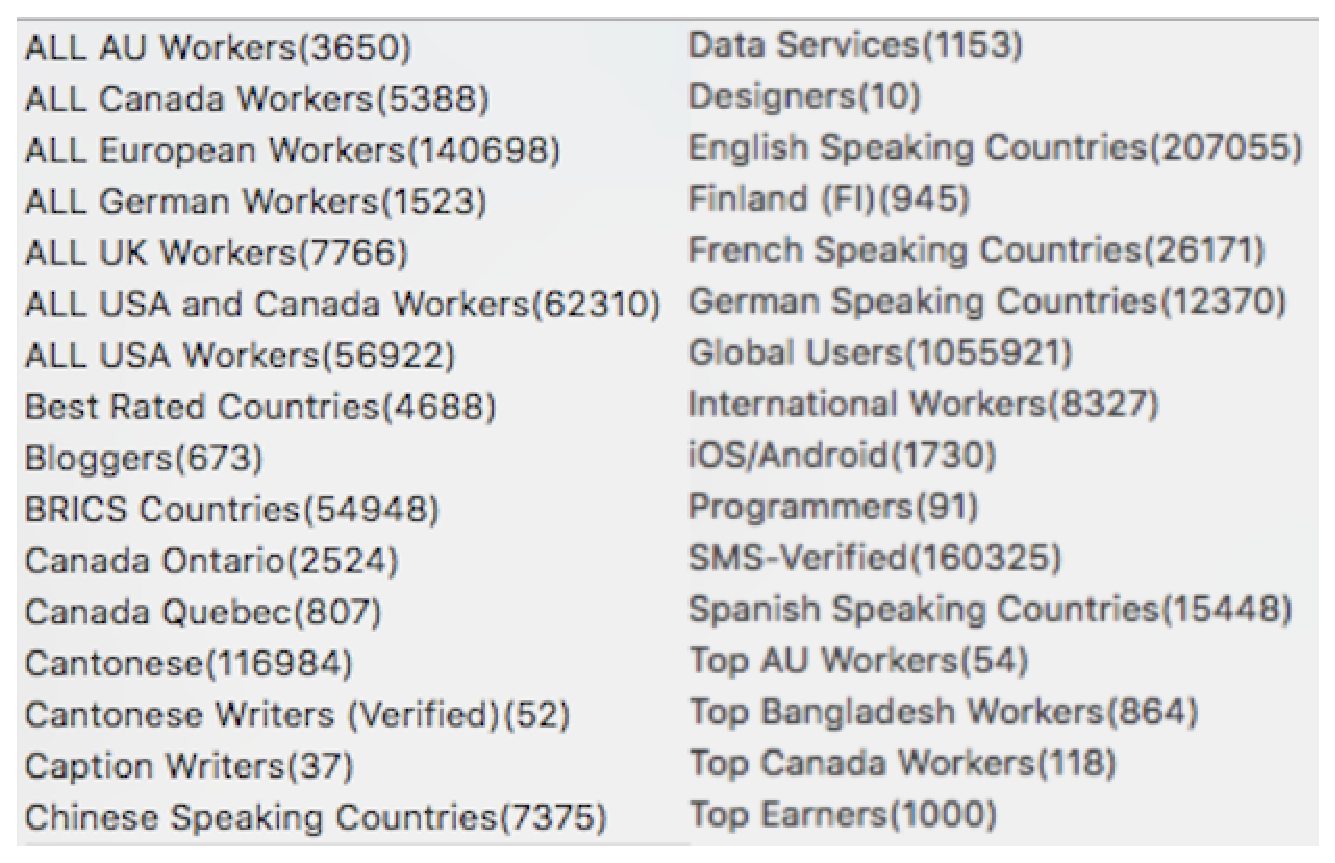
\includegraphics[scale=0.25] {figure/groups}}
%	\caption{Microworkers Hired Groups}
%	\label{groups}
%\end{figure}

The purpose of this paper is to use unskilled workers, although it was necessary for them to know enough of the English language to understand the video used in the experiment. For that reason, the tasks were launched as campaigns that used contracted groups, to increase the chance of the workers who contributed in a task also participate in others, was chosen a group of moderate size and with workers relatively assiduous so that the contributions were made quickly. The group chosen was Data Services, with 1153 potential workers to accept the jobs.

Some groups are made up of workers who only accept tasks that offer slightly larger payments, but considering the group chosen, it was feasible to offer a payment of 0,02 USD per task. Also, each task was active for 24 hours to reach all time zones in the same way.


\subsection{Planning}

The planning step has started with the identification of the microtasks needed to achieve the expected result. Since the goal was to generate enriched videos through supplementary content at points of interest, it was determined that they were needed. Thus, it was determined that four microtasks would be performed by the crowd:

\begin{itemize}
\item Identify the points of interest in the video; 
\item Gather content suggestions for each point of interest; 
\item Select the best extra content to each point of interest;
%Determine the most accepted supplementary content for each point of interest; 
\item Position the trigger items at the best spot over the video. 
\end{itemize}

Related to the items distributed to be annotated in each task, a circular list policy was adopted. In this way, there was a greater chance of each task, each item being annotated received the same number of contributions.

It was also necessary to determine how the video should be segmented to generate the input of the first task. The strategy chosen was to target the video based on the automatic captions generated by Youtube\footnote{https://youtube.com}. In this way, it was possible to generate short segments, but they tend to contain complete sentences. This method divided the video into 13 segments.

For budget and time issues, it was determined that the minimum amount of contributions each item could receive was five, so \textit{Task 0} should receive at least 75 contributions. The number five was chosen because it is odd, which avoids drawings, and because it is an amount that already allows seeing a tendency of convergence of opinion in a heterogeneous multitude.



\subsection{Production}
In this section will be described the 4 annotation tasks, as well the annotation tools, aggregation methods and results for each of them. Because there is a dependency order between these tasks, it's not possible run them in parallel. In this way, an execution workflow in which the output of one task is used for the next one, as can be seen in Figure \ref{workflow}.
%\begin{figure*}[h]
%	\centerline{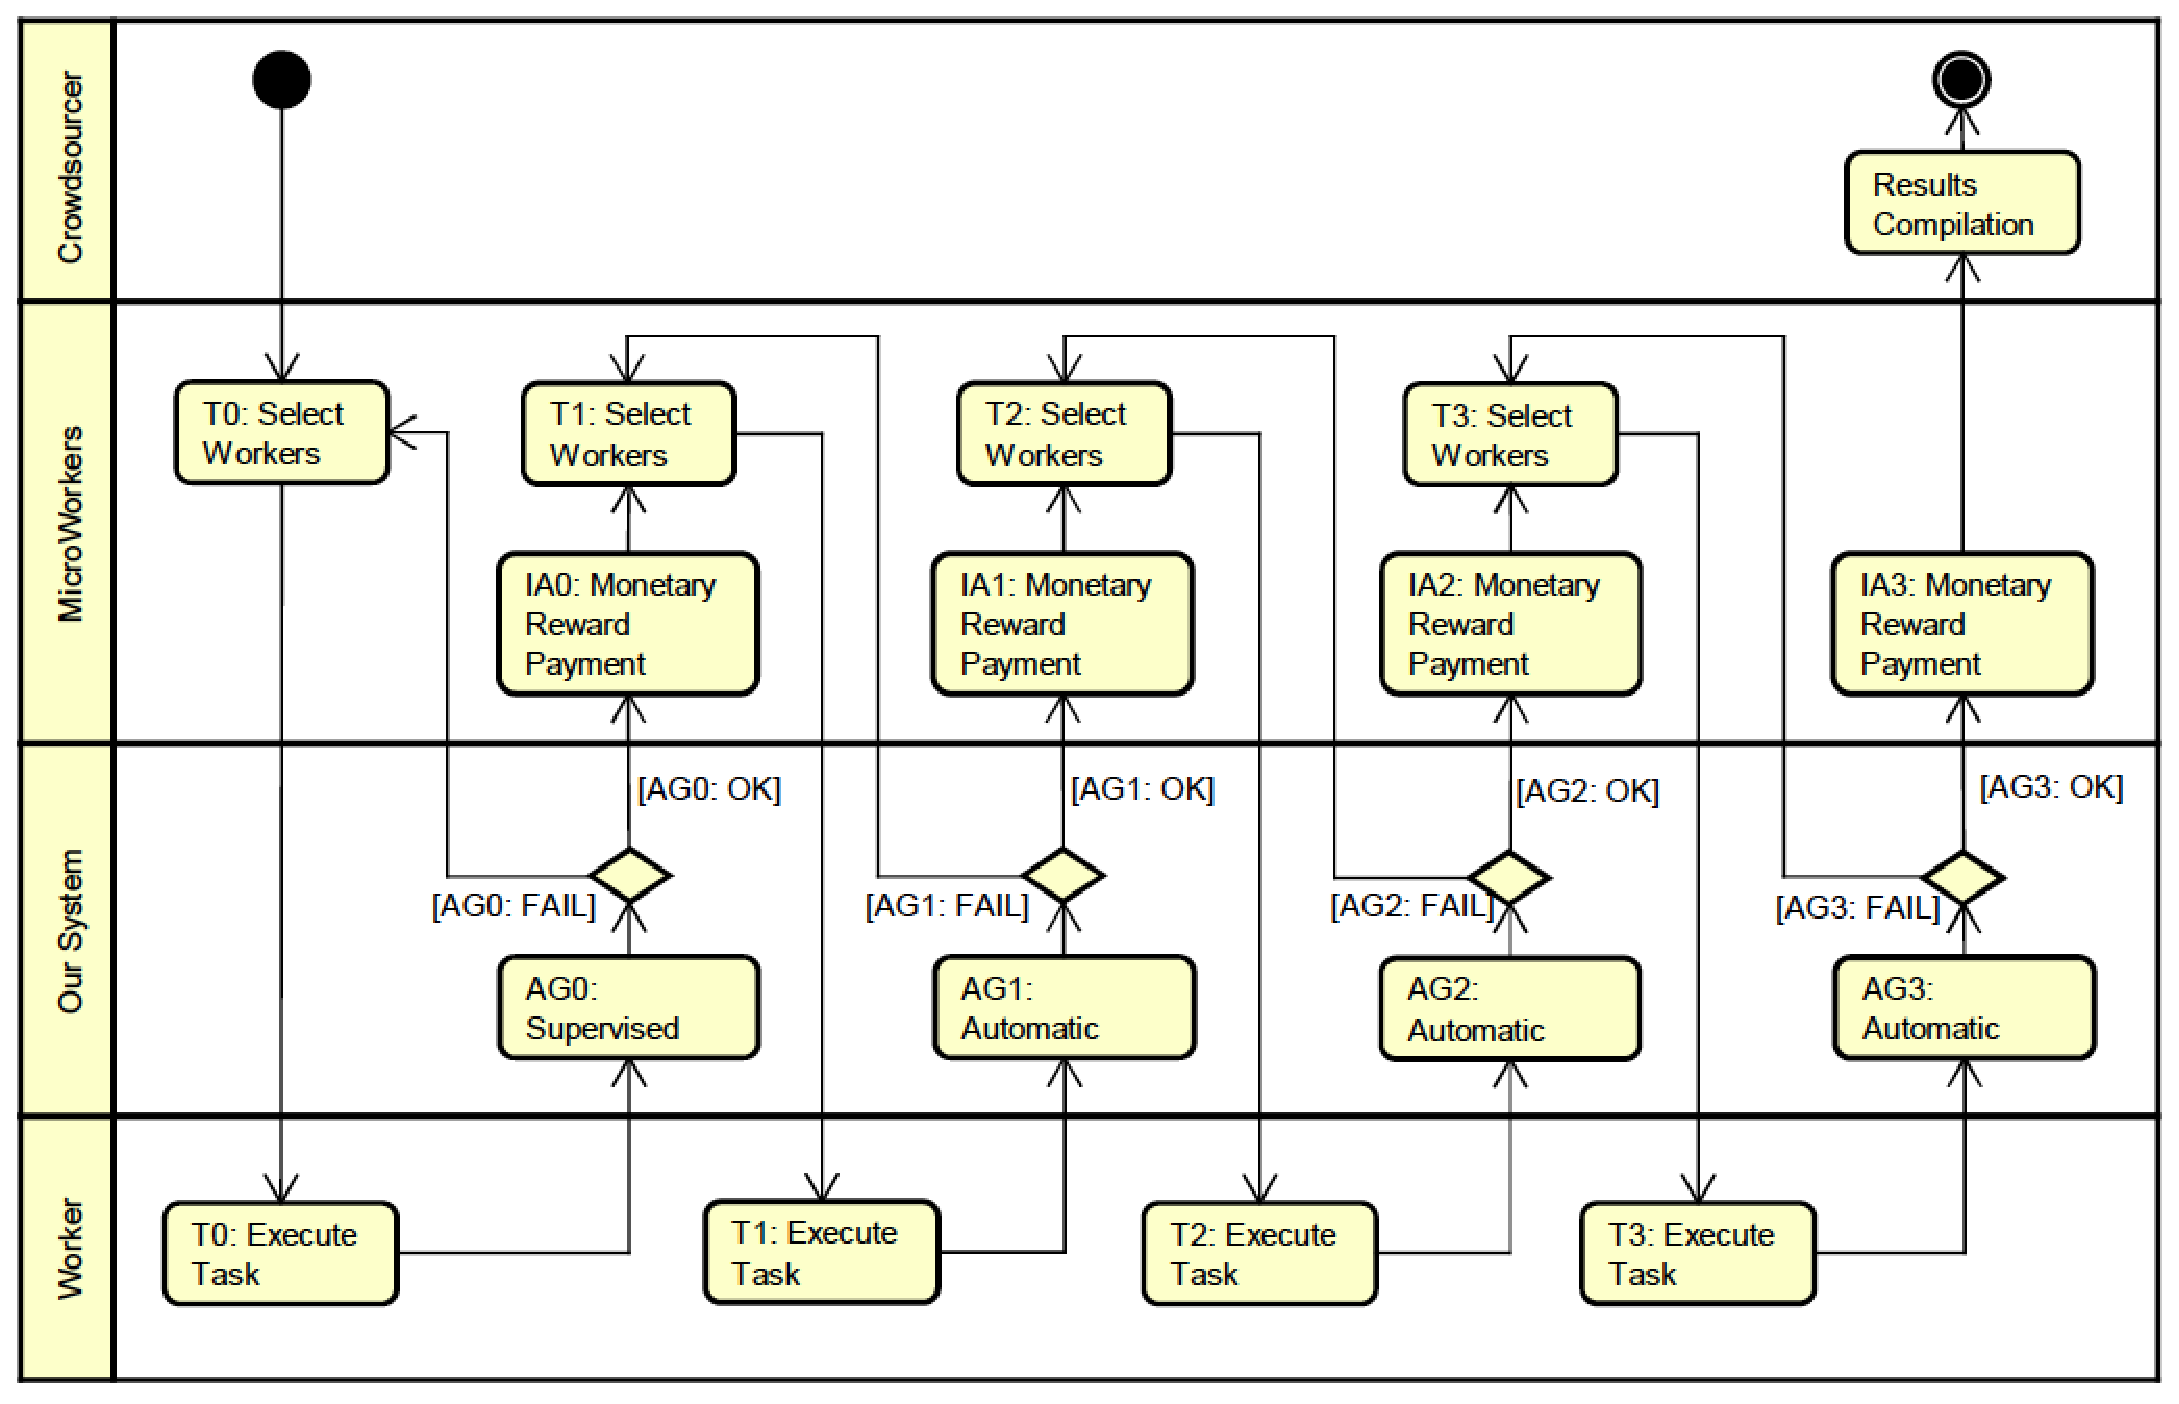
\includegraphics[scale=0.235] {figure/case}}
%	\caption{Video Enrichment Workflow}
%	\label{workflow}
%\end{figure*}

%Each of the four tasks applied to the workers will be described below, as well presented the annotation tool used for them.

\subsubsection{Task 0}
%\textbf{Identify Points of Interest:} The first annotation microtask is supported by the tool represented in Figure~\ref{task_1}, collecting identification for points of interest. In this task, the contributor receives a segment of video that should be watched, and if was found any point of interest, it should be marked and briefly described. These points of interest can be gestures, words, expressions, facts, concept, characters, events or anything that can be related to extra content.


\begin{itemize}
\item \textbf{Title:} Identify Points of Interest.

\item \textbf{Description:} A video segment is displayed to the worker and he must identify the moment at which a point of interest appears or is mentioned. This point of interest can be a person, a technology or a theory.

\item \textbf{Objective:} Identify points of interest in a video segment.


\item \textbf{Input:} A dataset with 13 video segments of 4.5 to 7 sec.


\item \textbf{Output:} A set of points of interest and the instant when they happen. In addition to serving as input to Task 1, this result also generated a summary based on points of interest.


\item \textbf{Instructions:} \begin{enumerate}
	\item Identify in the video something that you found interesting.
	\item Pause the video the moment it appears.
	\item Select its type: Person, Technology or Theory.
	\item Write what you have identified. 
\end{enumerate}

\item \textbf{Annotation Tool:} This tool (Figure~\ref{task_0}) receives information about the video segment to be displayed to the worker. The video is hosted on YouTube for the player to be created using the official API\footnote{https://developers.google.com/youtube/v3}. A timeline control has been implemented that ensures that the worker can use the features of the YouTube player, but only the interval related to the segment to be annotated is reproduced. The worker also has fine tuning buttons to position the video at the exact moment you identify the point of interest, a list with the category options (Person, Theory, and Technology) and the buttons to view the instructions and send the contribution.
\begin{figure}[h!]
	\centerline{\includegraphics[scale=0.17] {figure/task_0}}
	\caption{Annotation Tool for Task 0}
	\label{task_0}
\end{figure}

\item \textbf{Aggregation:} For this task, a supervised aggregation method was chosen in which the human interaction occurs at the end of the process. The contributions are filtered discarding the useless contributions (empty, nonsense, bad works), and the valid contributions are candidates to Points of Interest. The candidates are grouped in two-seconds interval ranges. In each group, a similarity analysis is done and the most frequent occurrence is selected. Finally, the human supervisor edits the selected label so that the text is visually pleasing. The aggregation method extracted 11 Points of Interest from the 75 contributions.

\end{itemize}



\subsubsection{Task 1}

%\textbf{Provide extra content suggestions:} The second task took as input the aggregated result from the task 1 that is a list of points of interest identified by the workers. This microtask is supported by the annotation tool represented in Figure~\ref{task_2}. This tool presents to the worker a point of interest and the video segment positioned at the moment it occurs. This way, is possible to use the video for reference and contextualization.



%Through this tool, the worker can contribute by writing a text related to the point of interest, sending an image or sending a link to a YouTube video or a Wikipedia page.


%When the collection of contributions for this task is done, the Aggregator groups the content of the sender by a point of interest, and then joins the similar suggestions. In this way, a list of points of interest with a set of content suggestions for each is added to the next task, without repeated suggestions.

\begin{itemize}

\item \textbf{Title:} Provide Suggestions for Extra Content.

\item \textbf{Description:} In this task, the worker receives a point of interest and the video synchronized at the moment it occurs. The worker should suggest extra content to complement the video, which may be a short text, an image or a link to a YouTube video or a Wikipedia page.

\item \textbf{Objective:} Obtain from the crowd extra content to each point of interest.


\item \textbf{Input:} The set of points of interest collected in \textit{Task 0}.


\item \textbf{Output:} A set of extra content associated with each point of interest. Each extra content may be an explanatory text, an image, even a link to a Wikipedia page or a Youtube video. Besides feed the \textit{Task 2}, this output is also used to generate a content-based index to the video.


\item \textbf{Instructions:} \begin{enumerate}
	\item Select the type of content to send.
	\item You can upload an image, write a short text.
	\item You also can paste a link to Youtube or Wikipedia.
\end{enumerate}

\item \textbf{Annotation Tool:} This tool (Figure~\ref{task_1}) receives information about the video segment, a point of interest present and the instant the point of interest occurs. The worker can use the player to play the video segment and understand the context of the point of interest, which is displayed in a text area at the top of the tool. He can select an option related to the kind of extra content they will provide, and according to this is displayed in a text field to paste a link or type a text, or a button is displayed to send an image. There is also a button to view the job instructions and a button to send the contribution.
\begin{figure}[h!]
	\centerline{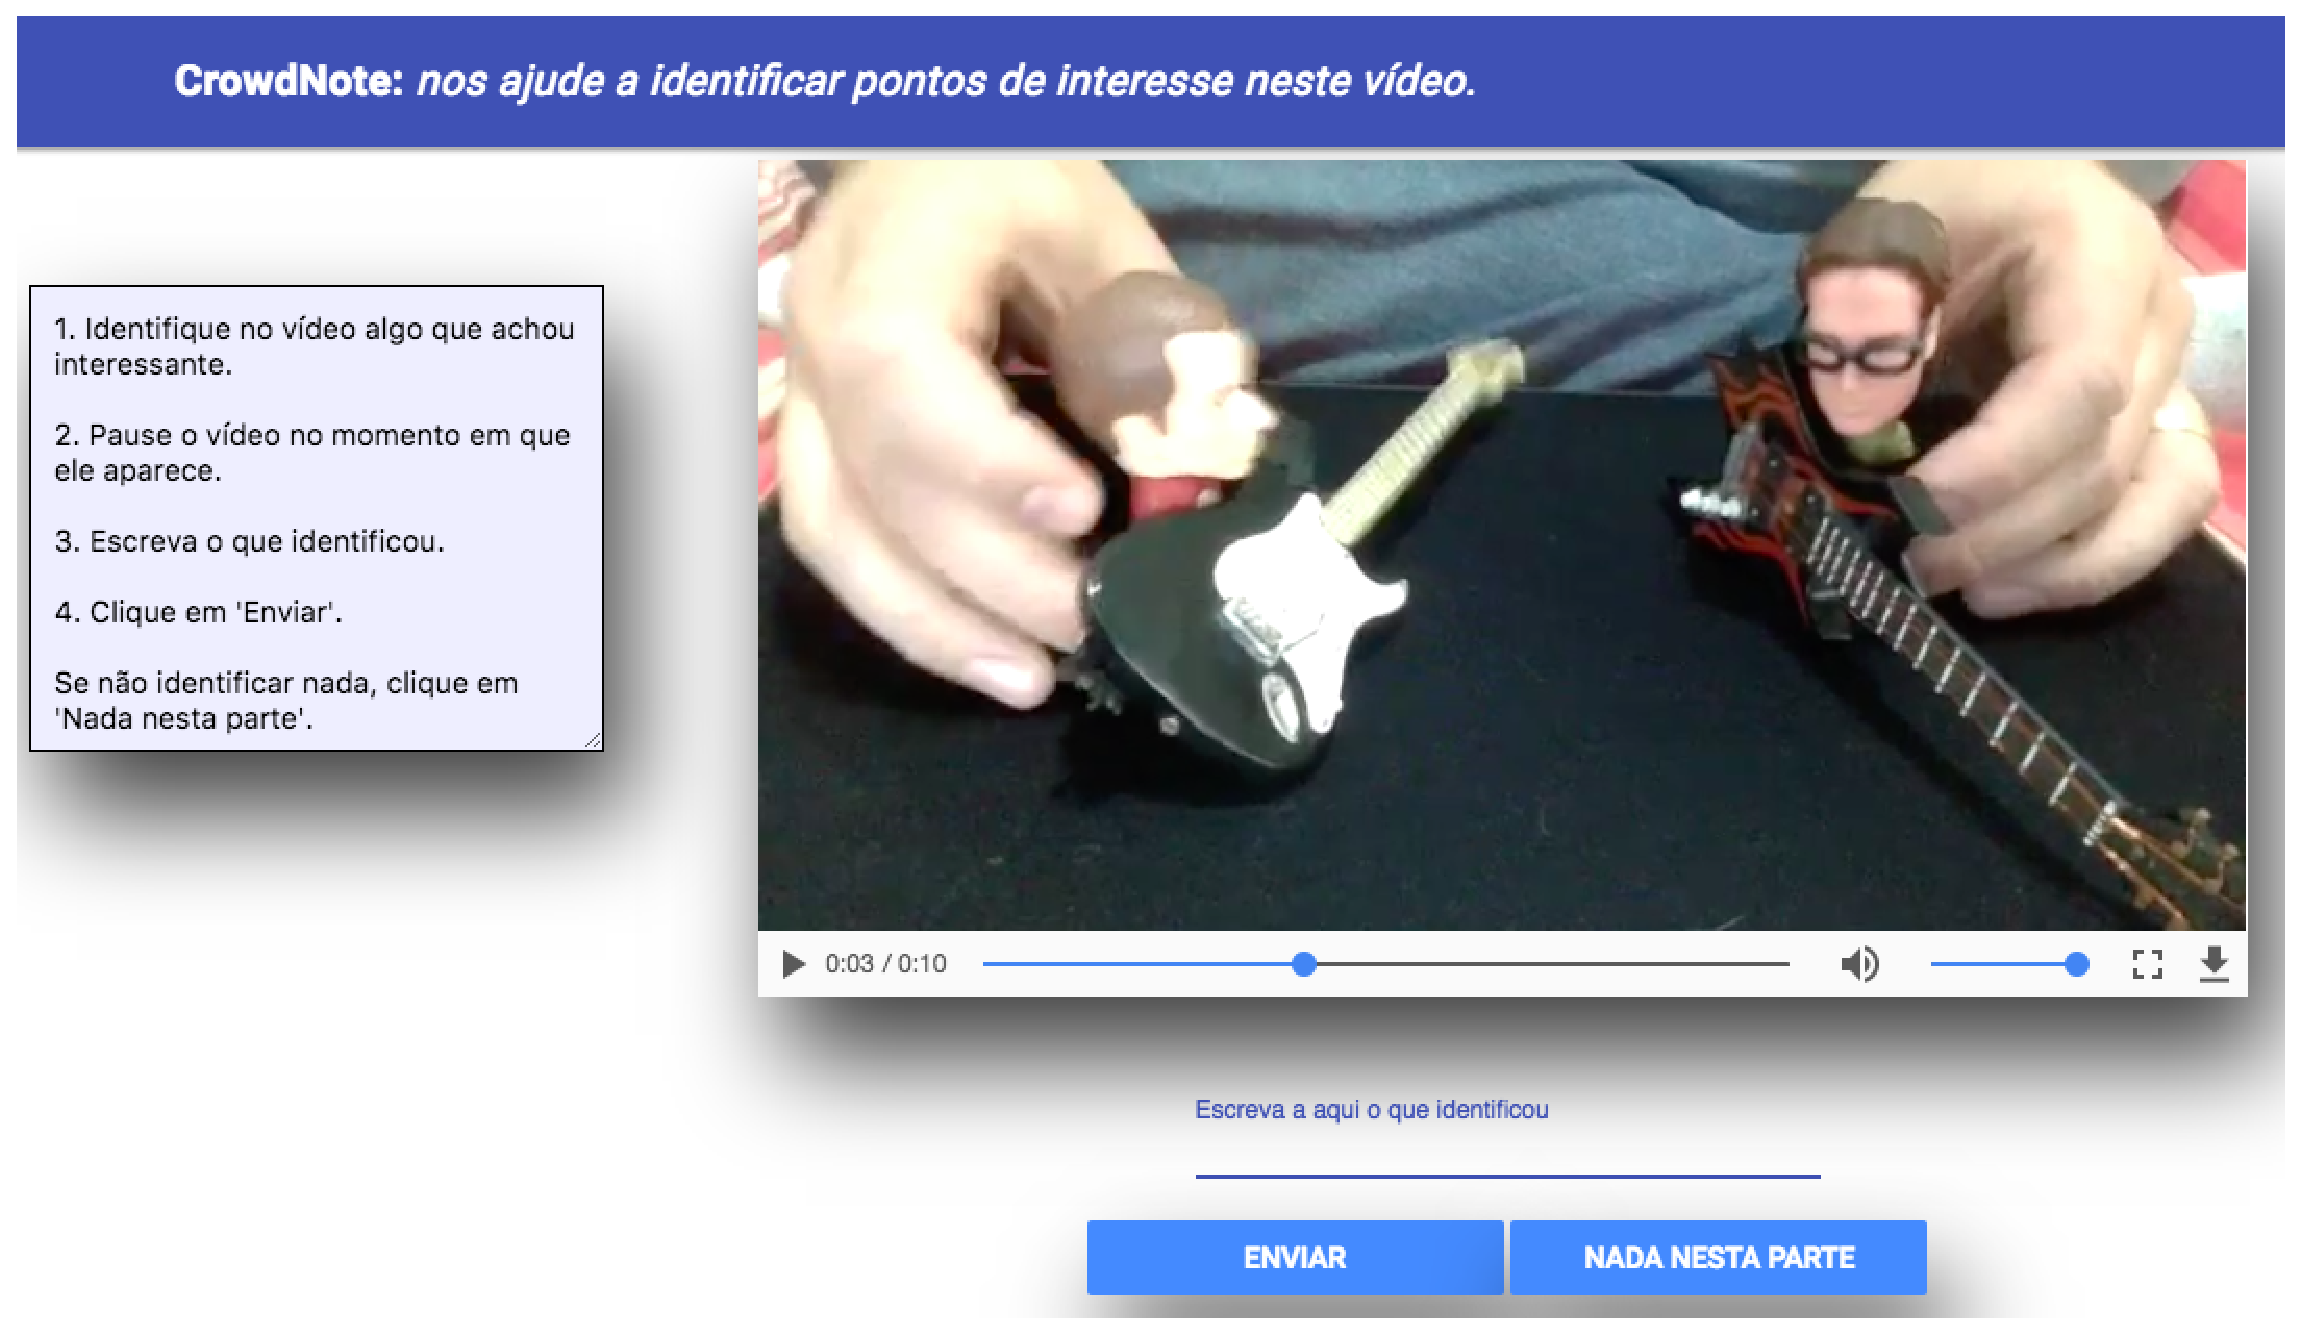
\includegraphics[scale=0.155] {figure/task_1}}
	\caption{Annotation Tool for Task 1}
	\label{task_1}
\end{figure}

\item \textbf{Aggregation:} For this task was chosen an automatic aggregation method. The filtering step discarded the corrupted files and broken links. The suggested contents were grouped by point of interest, and the duplicated items were merged. The aggregation method extracted 34 different suggestions of extra content from the 55 contributions received. All 11 points of interest received at least two content suggestions, some of which received four or five. 
%The ideal case would be to obtain a more even distribution, although the result obtained was enough to continue the process.

\end{itemize}


\subsubsection{Task 2}



\begin{itemize}

\item \textbf{Title:} Ranking Suggestions.

\item \textbf{Description:} The worker receives a point of interest and the video positioned at the moment it occurs. It also gets the list of suggested extra content to complement this point of interest. The job is to choose the extra content that best complements the content related to the point of interest.

\item \textbf{Objective:} Determine the best extra content to each point of interest, according to the crowd.


\item \textbf{Input:} A set of points of interest, with the suggested contents associated with each one.


\item \textbf{Output:} An updated set of points of interest with the extra contented associated with each one. This output also can be used to generate a ranked list of alternative extra contents to supplement the points of interest.


\item \textbf{Instructions:} \begin{enumerate}
	\item Use the buttons bar to navigate through the contents.
	\item You can use the zoom button to visualize each content.
	\item Vote for the content you liked best.
\end{enumerate}

\pagebreak

\item \textbf{Annotation Tool:} This tool (Figure~\ref{task_2}) receives as input the information relating to the video segment, the point of interest and a set of suggestions for extra content for it. The worker can browse content suggestions through the navigation buttons and can better visualize the content suggestions by clicking the zoom button. He can also play the video segment to understand the context of the point of interest. There is also the button to see the instructions and also the button to vote for the content you have chosen.

\begin{figure}[h!]
	\centerline{\includegraphics[scale=0.155] {figure/task_2}}
	\caption{Annotation Tool for Task 2}
	\label{task_2}
\end{figure}

\item \textbf{Aggregation:} This simple automatic aggregation method determines the most popular extra content suggested to each point of interest. As the contents were associated with 11 points of interest, were collected 55 contributions. In the filtering step the suggestions without votes was discarded. Finally, was generated an output with all 11 points of interest and the extra content associated with each one. 

\end{itemize}



\subsubsection{Task 3}

\begin{itemize}

\item \textbf{Title:} Determine the Position of the Trigger Items.

\item \textbf{Description:} This task consists of placing a trigger item in a video scene. This trigger item is represented as a rectangle containing a text or an image and should be positioned so as to minimize occlusions of important scene objects.

\item \textbf{Objective:} Determine the best position to display each trigger item over the video.


\item \textbf{Input:} A set of points of interest with the extra content associated with each one of them.

\item \textbf{Output:} Aset of points of interest with the extra content associated with each one, including now the position where each item should be displayed over the video. These positions are represented as coordinates (X,Y). The output of this task is the outcome of the video enrichment process, and can be executed in the Player. In addition, the metadata can be used to generate alternative outputs such as NCL to reproduce them in digital TV environments.


\item \textbf{Instructions:} \begin{enumerate}
	\item Drag the item by the video until finding the best position.
	\item When you have decided on the best position, click send.
\end{enumerate}

\pagebreak

\item \textbf{Annotation Tool:} This tool (Figure~\ref{task_3}) receives the information related to a point of interest and the video segment in which it occurs. This tool has a drag-and-drop feature that lets you drag the item through the video until you find the appropriate position. Using this feature, the worker can move the item over the video to find the position that looks best, avoiding occlusions of important scene objects.

\begin{figure}[h!]
	\centerline{\includegraphics[scale=0.17] {figure/task_3}}
	\caption{Annotation Tool for Task 3}
	\label{task_3}
\end{figure}

\item \textbf{Aggregation:} The automatic aggregation method applied at the final of this task determines the position at each item should be displayed over the video. The contributions for each item were grouped and the very discrepant positions of the others were discarded. Then, for each item, the average geographic position was calculated based on the X and Y coordinates predicted in the contributions. Was collected 55 contributions, of which 38 were after filtering. Of these 38 contributions were extracted the positions of the 11 items related to the points of intersection.

\end{itemize}


\subsection{Delivery}

Since this experiment aimed to generate enriched videos, the delivery of the outcome was done through a presentation system. This presentation system, shown in Figure~\ref{player}, receives the video, extra content, and necessary metadata from the Player Provider. This system is capable of reproducing the original video synchronized with the extra content, that is displayed every time a point of interest happens in the video. Is important to remind that all extra content displayed with the video was provided, selected and positioned by the crowd.



\begin{figure}[h!]
	\centerline{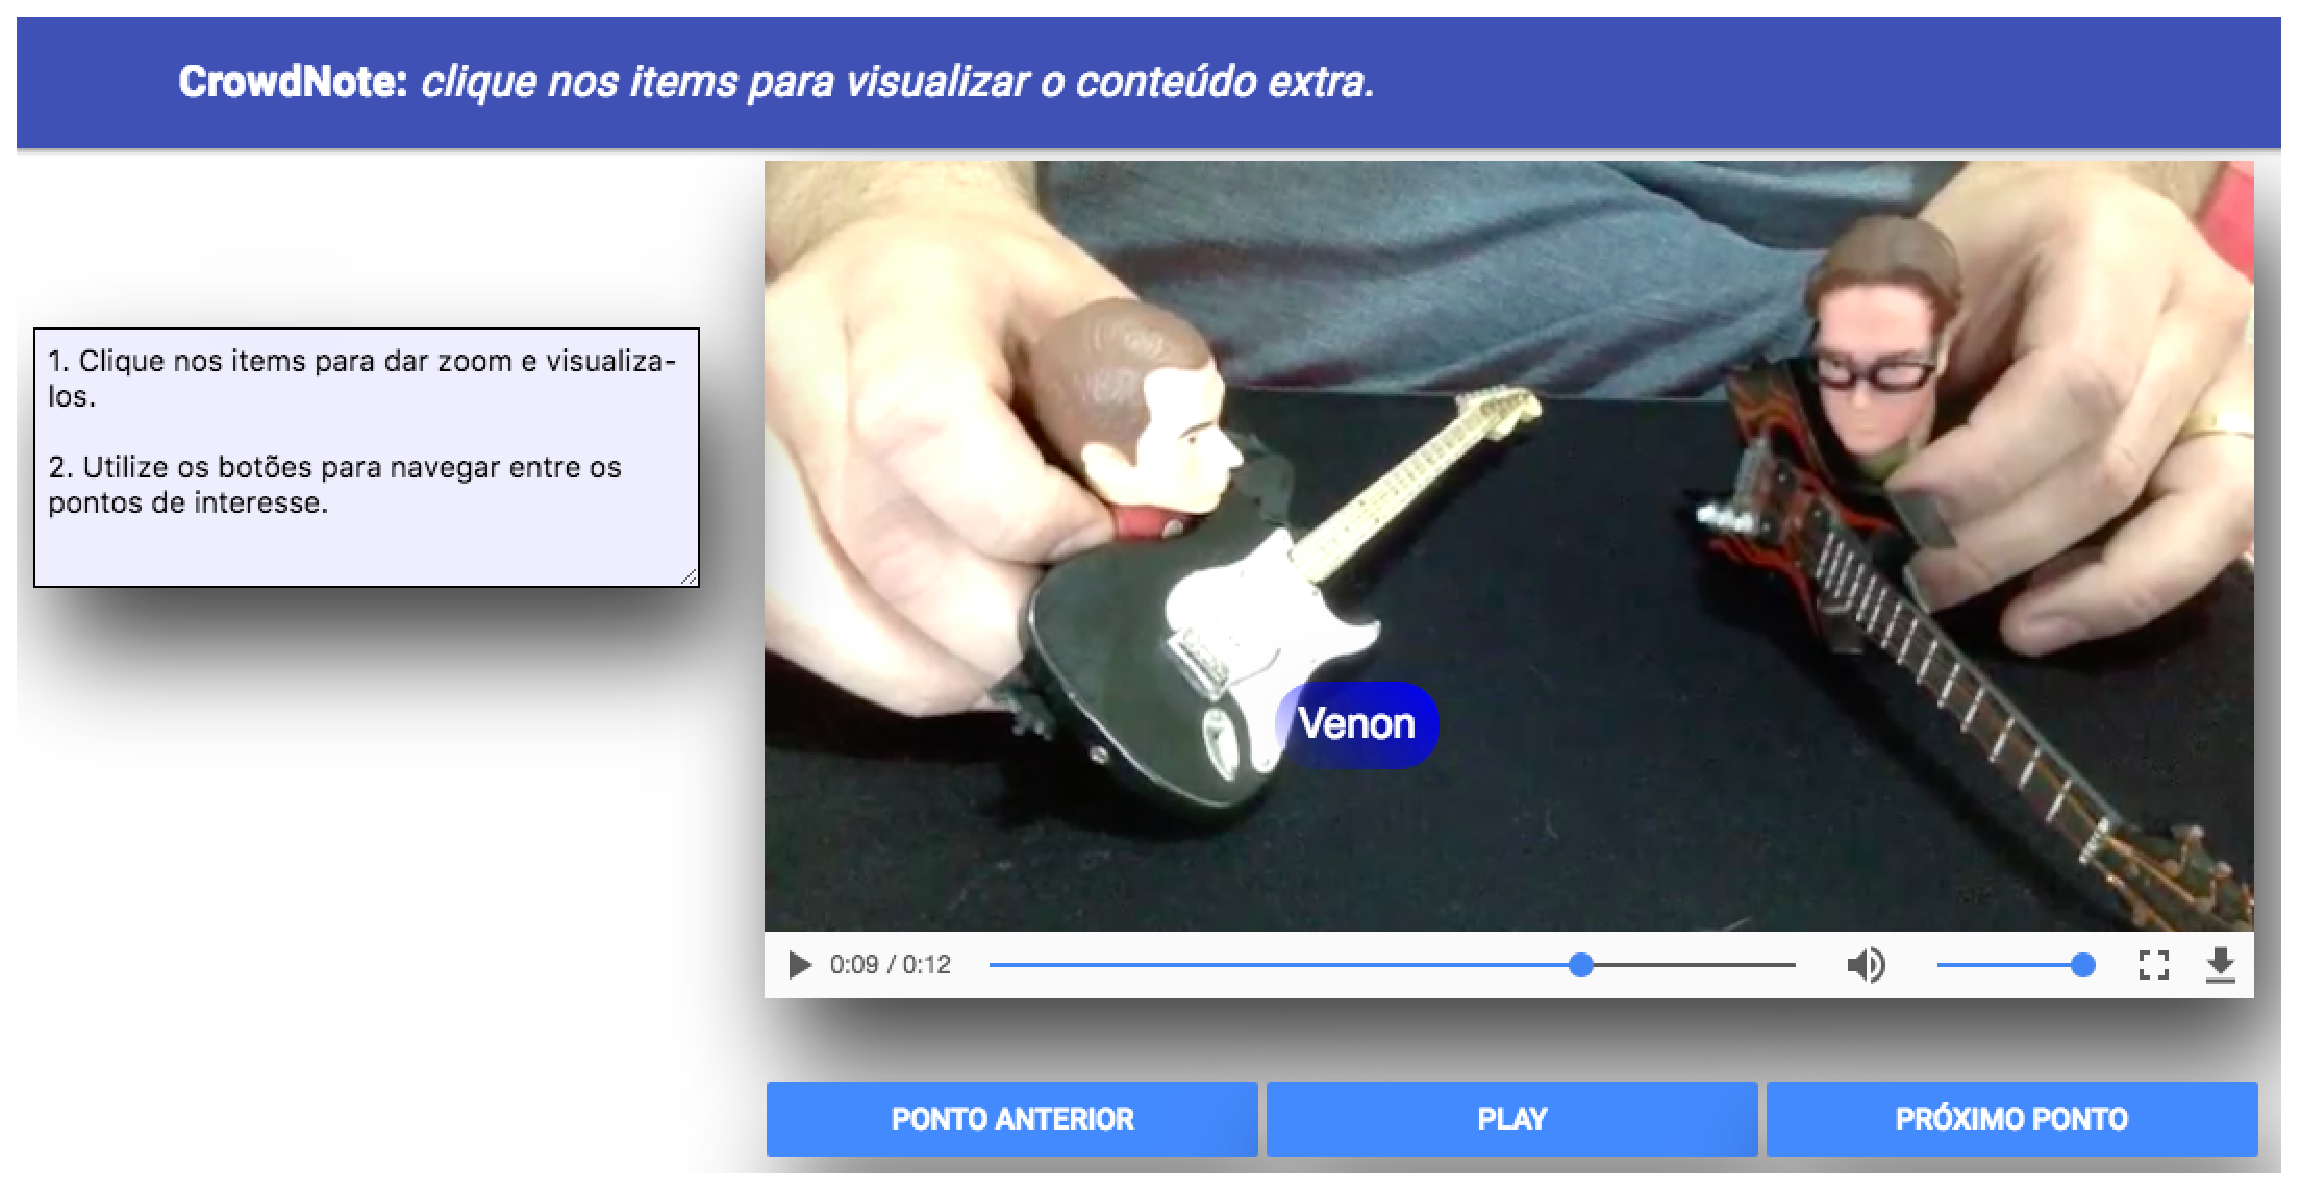
\includegraphics[scale=0.17] {figure/player}}
	\caption{Displaying an extra content item over the video}
	\label{player}
\end{figure}

This tool has a control bar with 3 buttons: Previous, Next and Zoom. These buttons are used to control two useful features, the content zoom and the navigation by point of interest.

The navigation by point of interest uses the list of points as a content index, allowing the user to navigate between points of interest by clicking the Previous and Next buttons. The Player automatically syncs the video at the time the current point of interest occurs.


When the user clicks the trigger item or the Zoom button, the extra content associated with the current point of interest is displayed on an upper layer as the video is paused. When you close the extra content, the video resumes its execution from where it was. The zoom view can be seen in Figure~\ref{player_zoom}.

\begin{figure}[h!]
	\centerline{\includegraphics[scale=0.17] {figure/player_zoom}}
	\caption{Player Zoom}
	\label{player_zoom}
\end{figure}



 \subsection{Runtime Observations}
 
During some tasks, we observed some interesting facts about the behavior of workers. Keeping in mind that the motivation of the workers in the experiment was the payment and that the amount paid for each job was small, the workers tended to do the bare minimum. This aspect proved to be correct that the decision was made to use microtasks that needed only a simple interaction to be completed.
 
The reflection of this led to some decisions during the experiment, as in Task 1. In this task, the worker were asked to suggest extra content to supplement the points of interest and for this, he could write a short text, paste a link to Wikipedia or Youtube, or upload an image. Most workers provided links and only two uploaded images. We thought that the reason was because sending an image was more laborious than pasting a link into the text box, as it was necessary to download the image and upload it.

However, this occurrence was used positively, because few image was obtained in the contributions, so, decided to add an automatic mechanisms to retrieve them automatically during aggregation. In cases where the selected point of interest was a Wikipedia link mechanism, it retrieved the main page image and, in cases where it was linked to YouTube, the thumbnail was retrieved from the video.

Although this operation is simple, it shows that it is possible to improve the aggregation methods by associating more automatic processing with human contributions. In this way, aggregation methods may be possible integration points with other systems, even with secondary human tasks to create a formal model of supervised aggregation activity.

\pagebreak


\subsection{Result Evaluation}
The rich video generated is a self-contained multimedia document, so the user doesn't need to access supplementary content from other sources.

Each supplemental content can be accessed through trigger items that are images and labels that appear in scenes where the point of interest is mentioned. When the trigger items are clicked, the video pauses the extra content is displayed so they can be viewed, and when closed, video playback resumes normally.

This outcome was evaluated according three criteria: points of interest identified, suitability of the associated content, and occlusion of scene objects.

According to the author of the video used in the experiment, there were 21 different points of interest, which after aggregation would result in 14, because at each interval of two seconds, only the most relevant point of interest would be selected. The crowd managed to identify 19 points of interest, which after the aggregates generated 11 relevant points. However, the crowd highlighted the term "Formalism" that  was not predicted by the author, who after checking it reported that it was valid in the video's context.

The extra content selected for each point of interest was also verified by the author. Of these, only one content did not meet the author's expectations. The content selected for "Logical relations and properties" corresponded to what the author wanted to convey. However, he realized that there was a flaw in the video script and the correct text would be "logical relational and its properties". This way this error can not be attributed to the crowd.

In relation to the occlusion of the objects of the scene, the criterion to calculate items that were positioned in the actress who narrated the text. Of the 11 items, only 2 slightly obscured the outline of the actress, as shown in Figure~\ref{oclusion}, but no item occluded her image significantly.

\begin{figure}[h!]
	\centerline{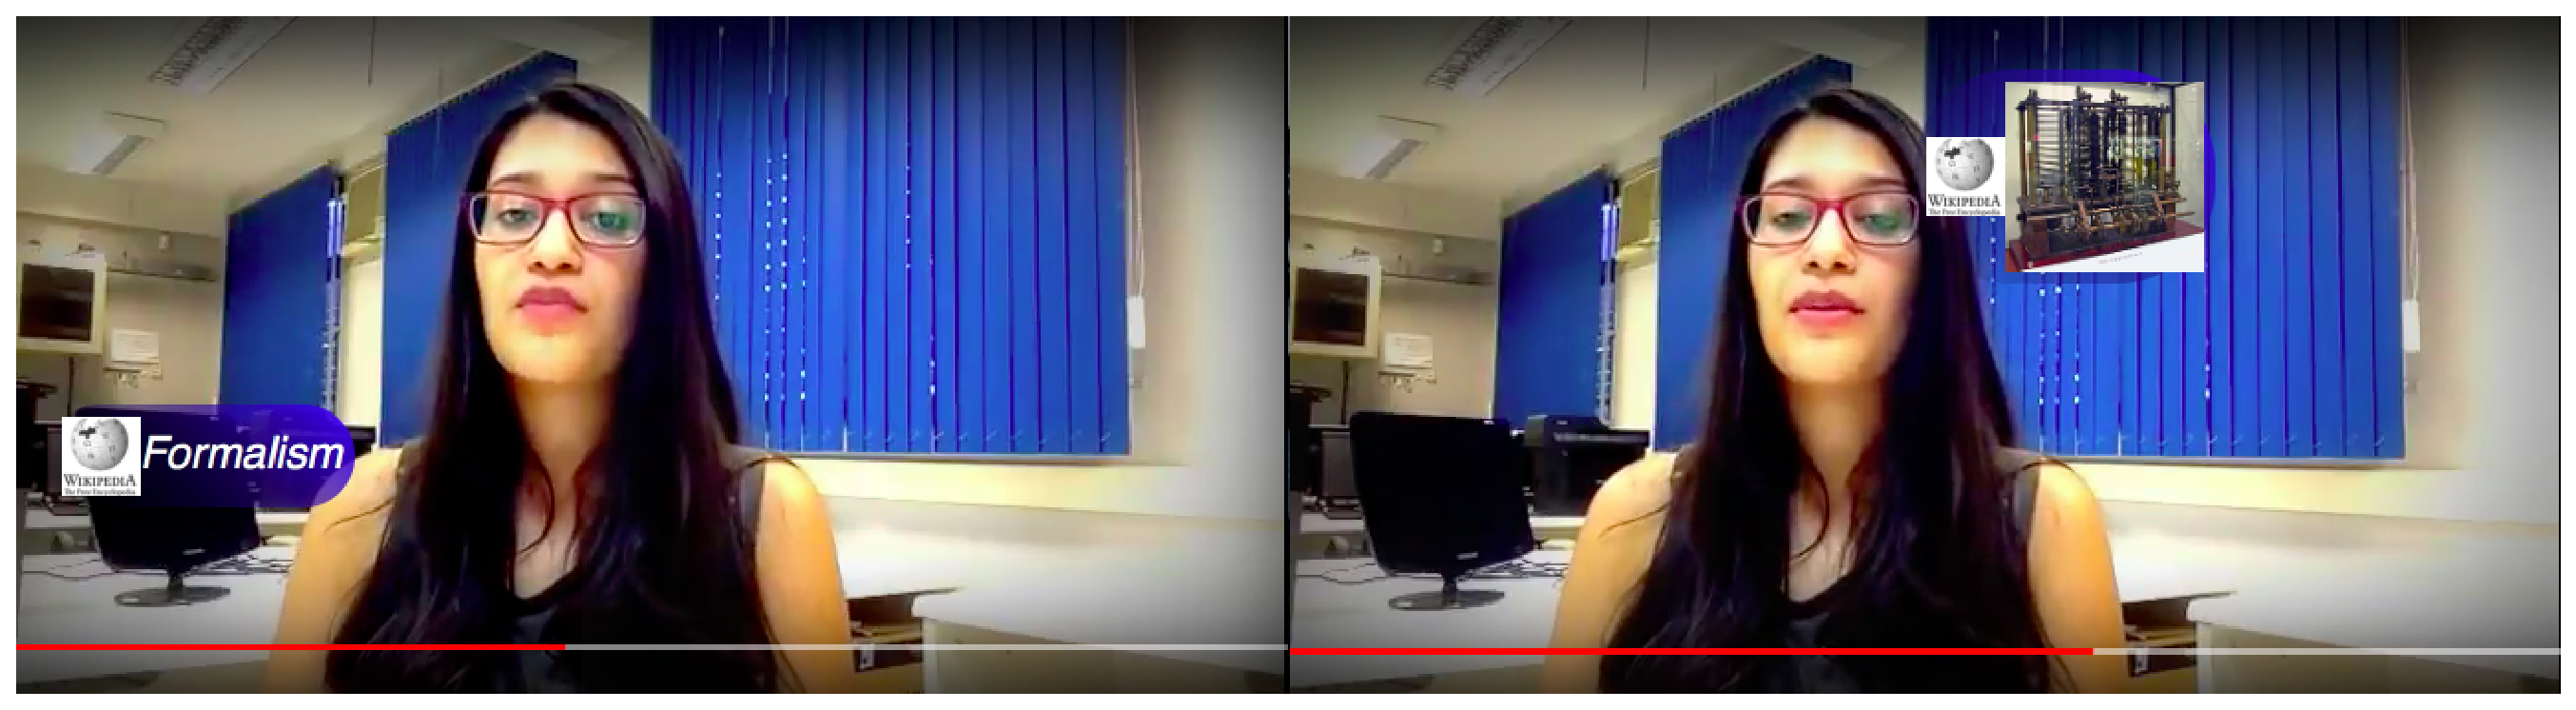
\includegraphics[scale=0.19] {figure/occlusion}}
	\caption{Occlusion Issues}
	\label{oclusion}
\end{figure}

In general, the result generated by the crowd was well adapted to convey the content intended by the author, having enriched virtually all the points that he had predicted. Finally, the result of our experiment demonstrate that the crowd is capable of generating dependable additional content to improve videos. The result of our case study can be seen in the player of our system\footnote{http://159.203.171.150:83}.



















